\documentclass[10pt,a4paper, titlepage, toc=idx]{scrreprt}

\usepackage[english]{babel}
\usepackage[utf8]{inputenc}
\usepackage{amsmath, amsthm, amssymb, amsfonts}
\usepackage{enumitem}
\usepackage{calrsfs}
\usepackage{mathtools}
\usepackage{mathrsfs}
\usepackage{nicefrac}
\usepackage{stmaryrd}
\usepackage{wasysym}
\usepackage{pifont}
\usepackage{wrapfig}

\usepackage{listings}

\usepackage{color}

\definecolor{mygreen}{rgb}{0,0.6,0}
\definecolor{mygray}{rgb}{0.5,0.5,0.5}
\definecolor{mymauve}{rgb}{0.58,0,0.82}

\lstset{ %
	backgroundcolor=\color{white},   % choose the background color; you must add \usepackage{color} or \usepackage{xcolor}
	basicstyle=\footnotesize\ttfamily,        % the size of the fonts that are used for the code
	breakatwhitespace=false,         % sets if automatic breaks should only happen at whitespace
	breaklines=true,                 % sets automatic line breaking
	captionpos=b,                    % sets the caption-position to bottom
	commentstyle=\color{mygreen},    % comment style
	columns=fixed
	deletekeywords={...},            % if you want to delete keywords from the given language
	escapeinside={\%*}{*)},          % if you want to add LaTeX within your code
	extendedchars=true,              % lets you use non-ASCII characters; for 8-bits encodings only, does not work with UTF-8
	frame=single,                    % adds a frame around the code
	keepspaces=true,                 % keeps spaces in text, useful for keeping indentation of code (possibly needs columns=flexible)
	keywordstyle=\color{blue},       % keyword style                 % the language of the code
	language=bash,
	morekeywords={*,...},            % if you want to add more keywords to the set
	numbers=none,                    % where to put the line-numbers; possible values are (none, left, right)
	numbersep=5pt,                   % how far the line-numbers are from the code
	numberstyle=\tiny\color{mygray}, % the style that is used for the line-numbers
	rulecolor=\color{black},         % if not set, the frame-color may be changed on line-breaks within not-black text (e.g. comments (green here))
	showspaces=false,                % show spaces everywhere adding particular underscores; it overrides 'showstringspaces'
	showstringspaces=false,          % underline spaces within strings only
	showtabs=false,                  % show tabs within strings adding particular underscores
	stepnumber=1,                    % the step between two line-numbers. If it's 1, each line will be numbered
	stringstyle=\color{mymauve},     % string literal style
	tabsize=2,                       % sets default tabsize to 2 spaces                  % show the filename of files included with \lstinputlisting; also try caption instead of title
	%	linewidth=80em,
}

\lstset{prebreak=\raisebox{-1ex}[0ex][0ex]
	{\ensuremath{\hookleftarrow}}}
\lstset{postbreak=\raisebox{0ex}[0ex][0ex]
	{\ensuremath{\hookrightarrow\space}}}

%\usepackage{lastpage}
\usepackage[svgnames]{xcolor}

%\usepackage{skriptum} % Layout and Design
% don't change the order of these or \i won't work as it should (I don't see why but that's how it is)
%\usepackage{cscallr} % Macros

\usepackage[T1]{fontenc}

\usepackage{charter}
\usepackage[bitstream-charter]{mathdesign} % imo nicer looking math font (fitting to the text font)
%\usepackage[expert]{mathdesign} % standard math font
\renewcommand*{\descfont}{\usefont{T1}{qhv}{b}{n}} 
\usepackage{fancyhdr, hyperref, titlesec, blindtext, color, subfigure}

%\usepackage{sectsty}
%\chapterfont{\usefont{T1}{bch}{b}{n}\selectfont\huge}

\hypersetup{hidelinks, linktoc=all,}

\newcommand{\HRule}{\rule{\linewidth}{0.5mm}}

\fancyhead[L]{\leftmark}
%\fancyhead[R]{\rightmark}
\fancyhead[R]{}
\fancyfoot{}
%\fancyfoot[L]{\emph{Skriptum Lineare Algebra I}} % name
\fancyfoot[C]{\thepage}
%\fancyfoot[R]{\emph{WS 2013/2014}} % semester
\pagestyle{fancy}
%headers
\renewcommand{\chaptermark}[1]{\markboth{\textsc{\chaptername\ \thechapter.\ #1}}{}}
\renewcommand{\sectionmark}[1]{ \markright{#1}{} }

% TOC
\usepackage[subfigure]{tocloft} % subfigure option only if using subfigure package
\renewcommand{\cfttoctitlefont} % ToC title
{\usefont{T1}{qhv}{b}{n}\selectfont\huge}
\renewcommand{\cftchapfont} % chapter titles
{\usefont{T1}{qhv}{b}{n}\selectfont}
\renewcommand{\cftsecfont} % section titles
{\usefont{T1}{bch}{m}{n}\selectfont}
\renewcommand{\cftsubsecfont} % subsection titles
{\usefont{T1}{bch}{m}{n}\selectfont} 
\renewcommand{\cftchappagefont} % chapter page numbers
{\usefont{T1}{bch}{b}{n}\selectfont}
\renewcommand{\cftsecpagefont} % section page numbers
{\cftsecfont} 
\renewcommand{\cftsubsecpagefont} % subsection page numbers
{\cftsubsecfont}

% chapter
\definecolor{gray75}{gray}{0.75}
\newcommand{\hsp}{\hspace{20pt}}
\titleformat{\chapter}[hang]{\Huge\fontfamily{qhv}}{\fontfamily{qhv}\bfseries\thechapter\hsp\textcolor{gray75}{$\vert$}\hsp}{0pt}{\Huge\bfseries}
% section
\titleformat{\section}[hang]{\Large\bfseries\fontfamily{bch}}{\thesection}{10pt}{\bfseries}
%subsection
\titleformat{\subsection}[hang]{\bfseries\fontfamily{bch}}{\thesubsection}{5pt}{\bfseries}

% theorems, not used in the linear algebra I script yet
\theoremstyle{definition}
\newtheorem{deff}{Definition}[section]
\theoremstyle{plain}
\newtheorem{propp}{Proposition}[section]

% macros
\renewcommand\over[2]{\genfrac{}{}{0pt}{}{#1}{#2}}

\newcommand*{\product}{Grit}
\newcommand*{\version}{1.0}
\newcommand*{\website}{\url{team-grit.com}}
\newcommand*{\repo}{\url{github.com/team-grit/grit}}


\begin{document}
%	\tikzstyle{every picture}+=[remember picture]
% \input{title.tex}
\begin{titlepage}
  \begin{center}
			
    % Upper part of the page. The '~' is needed because \\
    % only works if a paragraph has started.
    % \includegraphics[width=0.3\textwidth]{title_pic}~\\[1cm]
			
    % \textsc{\LARGE Grit}\\[1.5cm]
    
\includegraphics{grit}
			
    % Title
    \HRule \\[0.4cm]
    {\fontfamily{qhv} \huge \bfseries Using the\\\product{} Submission
      System \\[0.4cm] }
			
    \HRule \\[.5cm]
			
			
    {\small Official User Manual for Version \version}\\[1.5cm]
			
    
\includegraphics[scale=.25]{1024}
			
    % Author and supervisor
    % \begin{minipage}{0.4\textwidth}
    %   \begin{flushleft}
    %   \end{flushleft}
    % \end{minipage}
    % \begin{minipage}{0.4\textwidth}
    %   \begin{flushright}
    %     \large
    %     \emph{gelesen von:} \hfill
    %     Prof. Dr. Markus \textsc{Schweighofer}\\
    %   \end{flushright}
    % \end{minipage}
    % \large
    % \emph{Autor:} \hfill
    % Thomas \textsc{Schmidt}
			
    \vfill
			
    % Bottom of the page
    % {\large Sommesemester 2014}\\
    {\large \today}
			
  \end{center}
\end{titlepage}
\setcounter{tocdepth}{1}
	
\setcounter{page}{2} \cleardoublepage
\tableofcontents
\chapter{What is \product?}
%	\product{} offers a comprehensive solution for submission,
% fetching, evaluating and processing of programming course
% submissions. All you have to do is to press one button. The
% server-application constantly keeps an eye on associated
% repositories, e.g. \textsc{Ilias} and SVN, intelligently fetches
% student-submitted code and runs predefined tests. In the end, you
% receive a well-formatted PDF document or a plain-text file
% containing all the submissions of one assignment ready to print and
% hand over
% to your correctors.\\
%	Furthermore, \product{} lets you create overall statistics on
% score for one assignment, as well as for entire courses. Thus, it is
% easy to keep track on how your students perform.
\product{} is a system, developed by {\sc Team
  Grit}\footnote{\href{https://team-grit.com}{{\tt
      https://team-grit.com}}}, that makes the life of lecturers and
tutors of mainly programming courses easier and more comfortable. With
\product, we implemented a server-side one-button solution for
fetching and processing student submissions. This is done in such a
way that the tutors will not have to worry about not-compiling
programs and can therefore concentrate on the actually written code
and its quality. \product{} helps to maximize the teaching quality by
ruling out unnecessary work and lets the tutors focus on the really
important matter: Actual programming.
\section{What does \product{} do?}
With \product, the students do not directly submit their solutions to
our application. To be precise, they will not even notice that you are
using \product{} when submitting. Rather, \product{} fetches the student
submissions from whatever system provided for that purpose. As for
now, \product{} supports Subversion, Ilias and Email submissions,
however, because of its high modularity, you can easily add your own
{\it fetcher}. At the end of a previously set deadline,
\product{} fetches the submissions and processes them. As of now, we
support Java, C and Haskell submissions, but like {\it fetchers},
additional modules can be added. After the processing, which includes
compiling and testing the submission, using previously set unit tests,
we will put that acquired information about the submission in a
report, ready for you to download. For now that report will be either
a PDF or a plain-text file, but, as you will have guessed, other
formats can be implemented easily.
\subsection*{What \product{} does not.}
\product{} does not provide submission features, as it can only import
submissions. Also, it is not possible to manipulate code in \product,
because this is not what it was intended for: offline correction on
paper.  \product{} does not replace a lecturer or tutor by adopting all
of their correction procedure, however \product{} simplifies their work
in supporting them with automatable checking routines. So,
\product{} does not offer any methods to control semantical errors in
the program code like checking if the summation really does add the
two summands.  Furthermore \product{} is not suitable to test if the
submitted solutions of the students actually solves the given problem or
a part of it. \product{} cannot check any additional exercise
restrictions specified in the assignment paper (e.g. using inherited
methods for solving the exercise). \product{} will also not correct any
programming faults automatically, but will present you the incorrect
passage, the error, the passed tests as well as compiler
error message.
\section{When do you need \product?}
You are a lecturer/tutor of a general programming course, a java
workshop, a C++ seminar, ..., in which the participants can or have to
submit solutions to a given problem. If you are tired of searching for
syntax errors, compiling errors, typos, etc. for hours at a time, then
you will definitely appreciate our product to increase the efficiency
of your correction by prechecking every submitted solution. All in
all, if you are a university or college professor or lecturer,
teacher, tutor, or corrector, \product{} can help you automate
collecting electronically submitted assignments concerning programming
code from various resources. Compiling tests and predefined tests can
be run so you can easily focus on the important things.

\subsection*{When you don't need \product.}
You won't need \product{} if you do not provide electronic submission of
assignments for your course. Also, \product{} is only suitable for
fetching programming code assignments, however, other types of
submissions can be added by oneself.  \product{} does not offer any
features for students, as it only provides functionalities used by
teachers and correctors.
\section{What are the alternatives?}
\begin{itemize}
\item The Marmoset Project \\
  (\url{marmoset.cs.umd.edu}) \\
  Marmoset is a system for handling student programming project
  submission, testing and code review. It has been developing at the
  University of Maryland for over 5 years. It works in all different
  programming languages, and is designed to work well with both very
  small and very large projects, such as our OS course in which a
  submission consists of tens of thousands of lines of code.
\item BOSS Online Submission System (Beta phase) \\
  (\url{sourceforge.net/projects/cobalt}) \\
  BOSS is a course management tool that allows students to submit
  assignments on-line in a secure manner. Staff can mark work and run
  automatic tests on submissions.
\item Cafe grader \\
  (\url{gitorious.org/cafe-grader}) \\
  Cafe grader is a submission and grading system for programming
  contest and training.  This software was used in APIO'08. It
  currently has mainly two components: the web submission system and
  the grader. The web app uses Ruby on Rails; while the grader was
  written in plain Ruby. Current activity: process of migrating to
  git, and developing installation scripts.
\item Praktomat \\
  (\url{https://github.com/KITPraktomatTeam/Praktomat/})
  \\
  Praktomat is a quality control system for programming
  exercises. Students hand in their submissions directly into
  Praktomat which then compiles and tests them. It was first developed
  at the University of Passau in 1998 and was later migrated to the
  Karlsruhe Institute of Technology in 2008.  The software is written
  in Python and uses the Django web framework. It is able to manage
  Java, other programming languages can be added.
\end{itemize}
% writing modules yourself or using other software
\chapter{Getting Help}
There are various resources available to get most out of \product.
\section{Our Website}
On our website (\url{team-grit.com}), you will find links to latest
builds of \product{} as well as information on the new added features.
\section{Online Documentation}
The online version of the documentation is essentially the same as the
one you are reading now, however, you will have access to additional
resources concerning troubleshooting.
\section{Contact us}
Do you have suggestions? Do you miss a feature? Contact us through our
website \url{team-grit.com}.
\chapter{Getting \product}
As you are reading this documentation now, you have most likely
already acquired \product. It is either directly available by getting
it from the developers, or found on the associated GIT repository.
\chapter{Installing \product}
\product{} is normally delivered as a virtual machine, thus, this
chapter concentrates on running \product{} via this VM. If you wish to
run \product{} natively or on another virtual machine, you will find the
associated requirements
in \hyperref[4.3]{Section 3} of this chapter.\\
The advantage of using a pre-configured virtual machine is that
\product{} is able to run without making any changes. Only a minimum of
configuration, for example setting up the network, is needed. All
necessary components are already installed and \product{} is ready to
run.

\section{Importing the \product{} VM} \label{gritvm} How to import the
\product{} virtual machine depends on the used virtualization packages.
% if someone knows about other vm progs This section will cover the
% most commonly used ones and the settings that are required to run
% \product.
This section will only cover VirtualBox Version 4.0.x since it is one
of the most commonly used virtualization programs and is (mostly)
free\footnote{\href{https://www.gnu.org/philosophy/free-sw.html}{{\tt
      https://www.gnu.org/philosophy/free-sw.html}}}.  Still, the
settings made for VirtualBox also apply if you use other
applications, though details may differ.\\
First, the installation via command-line interface is encouraged since
you will most likely run the VM on a server without any graphical user
interface. After that, a short
guide for the VirtualBox graphical interface is given.\\
Importing and applying the settings via the graphical interface might
be a lot easier since you directly get to the VM login screen and
don't have to login via {\tt ssh} which might be not possible if the
network setting aren't correct, for which we can't take care of.
\subsection{Import into VirtualBox via Command-line}
The \product{} virtual machine image comes in the Open Virtualization
Format (OVF). First off, the VM needs to be imported using
\begin{lstlisting}
	$ VBoxManage import GritVM.ovf
\end{lstlisting}
This command imports the virtual machine with all its optimal settings
and you are ready to start it using
\begin{lstlisting}
	$ VBoxManage startvm GritVM --type headless
\end{lstlisting}
	
	\subsection{Import into VirtualBox via graphical Interface}
	To import the OVF file into VirtualBox using the graphical
        interface, go to "{\tt File > Import Appliance}" and choose
        the OVF file downloaded previously. Next, launch the VM either
        by double-clicking on it or selecting "{\tt Start}" on the
        menu bar.
        \section{Prerequesites}
        \subsection{SSH key permissions}
        Ensure that the virtual machine keyfiles are readable only by
        the current user. Otherwise SSH will refuse to use them. In
        order to set the proper permissions execute the command
\begin{lstlisting}
          sudo chmod 0700 -R /res/keyfiles 
\end{lstlisting}
        form the \product{} root folder.

        \subsection{SVN repository setup}
        If you plan to use an SVN repository a ``mapping file'' must
        be provided. This file maps the name of the student folders to
        the student email address. Create a file \texttt{students.txt}
        in the top level of the repository. This file should contain
        only blank lines or lines formatted like \texttt{StudentFolder
          = StudentMail}. Lines beginning with the
        ``\texttt{\#}''-sign will be ignored.

        The file might look like this:
\begin{lstlisting}
          # this is a comment
          stud01 = max.mustermann@test.de
          stud02 = elsbeth.musterfrau@test.de
\end{lstlisting}

	\section{First Startup}
	After the first boot, assuming you started the VM via
        command-line, it is necessary to log into the VM via {\tt
          ssh}. If you used the graphical interface, you can skip this
        first part on how to obtain the VM's dynamic IP and
        immediately read about how to setup the static IP since you
        are able to just login via the graphical interface.

	\subsection{Get the current dynamic IP of our VM}
	The IP address is required for this task. Since the VM is
        using a dynamic IP address by default (you will change that
        soon), you will not know this address beforehand. To find out,
        execute the following command on the host machine:
	
	\begin{lstlisting}
	$ VBoxManage guestcontrol GritVM exec --image /sbin/ifconfig
	--username grader --passwort grit!securedThisUser --wait-stdout
\end{lstlisting}
	
	This executes the {\tt ifconfig} command as the standard user
        called {\tt grader} with the standard password {\tt
          grit!securedThisUser} and waits for the command output to
        get printed. The output will look similar to the following:
\begin{lstlisting}
	eth0      Link encap:Ethernet  HWaddr 08:00:27:7c:36:06  
	inet addr:192.168.0.42  Bcast:192.168.255.255  Mask:255.255.0.0
	inet6 addr: 2a02:8071:8385:2601:a00:27ff:fe7c:3606/64 Scope:Global
	inet6 addr: fe80::a00:27ff:fe7c:3606/64 Scope:Link
	UP BROADCAST RUNNING MULTICAST  MTU:1500  Metric:1
	RX packets:47 errors:0 dropped:0 overruns:0 frame:0
	TX packets:65 errors:0 dropped:0 overruns:0 carrier:0
	collisions:0 txqueuelen:1000 
	RX bytes:6212 (6.0 KiB)  TX bytes:3482 (3.4 KiB)
	
	lo        Link encap:Local Loopback  
	inet addr:127.0.0.1  Mask:255.0.0.0
	inet6 addr: ::1/128 Scope:Host
	UP LOOPBACK RUNNING  MTU:16436  Metric:1
	RX packets:16 errors:0 dropped:0 overruns:0 frame:0
	TX packets:16 errors:0 dropped:0 overruns:0 carrier:0
	collisions:0 txqueuelen:0 
	RX bytes:1280 (1.2 KiB)  TX bytes:1280 (1.2 KiB)	
\end{lstlisting}
	You are concerned with the {\tt eth0} interface. In this
        output, right after the entry {\tt inet addr}, you can see
        that the VM is currently using the IP {\tt 192.168.0.42}. Now,
        you can log into this VM from a computer in the same network
        (or any computer if you already set up forwarding, which is
        not discussed in this document) using {\tt ssh}:
\begin{lstlisting}
	$ ssh grader@192.168.0.42 # internal or external ip
\end{lstlisting}
	\subsection{Basic Security}
	Now that you are logged in, it is highly recommended to change
        the user and root passwords. As you may have noticed, the
        password for the user {\tt grader} is {\tt
          grit!securedThisUser}. The {\tt root} password is {\tt
          root}. To change these, type the following:
\begin{lstlisting}
	$ passwd # change password of logged in user (i.e. grader)
	$ su # login as root
	% passwd # change root password
\end{lstlisting}
	If you want to add additional security to the {\tt ssh}
        server, you may want to generate a {\tt ssh} key and change
        the settings of the
	server so that you can only login via a previously added {\tt ssh} key.\\
	{\color{red} WARNING: If you lose that key you can NOT login
          via {\tt ssh} anymore. You will need direct access to the
          machine to
          disable the option and/or add the newly generated key!}\\
	To do this you need to generate your key on your local
        computer first and then copy said key into the VM using:
\begin{lstlisting}
	$ ssh-keygen -t rsa # create a rsa ssh-key
	$ ssh-copy-id grader@192.168.0.42 # copy your ssh-key into the
VM
\end{lstlisting}
	To disable password login on the virtual machine so that you
        can only login using your {\tt ssh}-key, you now need to login
        into the VM, edit {\tt /etc/ssh/sshd\_config} and change the
        {\tt PasswordAuthentication} entry to
\begin{lstlisting}
	PasswordAuthentication no
\end{lstlisting}
	This entry will already be there, however, it is commented
        out. You only have to remove the {\tt\#} to disable password
        logins.
	\subsection{Setup a static IP address}
	After your first login, you will have to setup the network
        according to your local setup and (probably) set a static
        IP. For that, you need to edit {\tt
          /etc/network/interfaces}. By default, the file looks like
        this:\pagebreak
\begin{lstlisting}
	# This file describes the network interfaces available on your system
	# and how to activate them. For more information, see interfaces(5).
	
	# The loopback network interface
	auto lo
	iface lo inet loopback
	
	# The primary network interface
	allow-hotplug eth0
	
	iface eth0 inet dhcp
	
	# iface eth0 inet static
	#	 address 192.168.0.42
	#	 netmask 255.255.0.0
	#	 gateway 192.168.0.1
\end{lstlisting}
	The important part - again - is the specification of the {\tt
          eth0} interface: Here, you first comment out where the {\tt
          eth0} interface is set up with a dynamic address ({\tt
          dhcp}) and instead use the pre-outcommented template below
        that. Then assign a static IP address,
	set the net mask and tell the VM what IP address your router has.\\
	After that, you need to reboot the VM by typing
\begin{lstlisting}
	$ sudo shutdown -r now$
\end{lstlisting}
	and you are done setting up the VM and are ready to launch
        \product.
	\section{Infos about the VM}\label{4.3}
	In this section, information is given about the VM \product{} is
        shipped with and how you have to configure your own system if
        you chose not to use the VM provided. Also, the configuration
        already predefined for running the provided VM via VirtualBox,
        for example which network setting to use, are given.
	\subsection{The System}
	The provided virtual machine is running Debian Wheezy 7.5
        64bit. It is a widely used, stable, performant, widely
        supported operation system, and very slim nevertheless. We did
        not provided a graphical interface since all configuration can
        be easily done via ssh. Furthermore, this saves memory and
        disk space. Tools like {\tt sudo} and {\tt apt-get} are
        already installed so that you are able to install additional
        tools and updates. The system settins made in the VM
        configuration set memory to 1GB of memory, 12MB of video
        memory, 8GB of virtual disk space and a bridged network
        adapter (e.g. Intel PRO/1000 MT Desktop).
	\subsection{Required Software}
	\product{} depends on several packages to be installed on the
        system for standard functionality. These are:
	\begin{itemize}
        \item OpenJDK 7 ({\tt openjdk-7-jre})
        \item Java Compiler ({\tt javac}) \\
          Note: You have to ensure that {\tt javac} is part of the
          system's PATH variable. This only concerns systems running
          Windows.
        \item TeXLive ({\tt texlive-full})
        \item PDF LaTeX ({\tt PDF LaTeX})
        \item GNU C Compiler ({\tt gcc})\\
          Note: You have to ensure that {\tt gcc} is part of the
          system's PATH variable. This only concerns systems running
          Windows.
        \item Glasgow Haskell Compiler ({\tt ghc6}) \\
          Note: You have to ensure that {\tt ghc6} is part of the
          system's PATH variable. This only concerns systems running
          Windows.
        \item Subversion ({\tt svn})
        \item Secure Copy ({\tt scp})
        \item G++ Compiler ({\tt g++})
	\end{itemize}
	All of the above packages resemble {\it latest}
        releases. These might not be available through {\tt apt-get}
        and need to be installed directly, this is, for example, the
        case for TeXLive.
	\section{ILIAS Virtual Machine}
        Since \product{} requires full access to ILIAS' database and
        file system, it is advisable to run a separate installation of
        ILIAS for use with \product{}. The courses in this ILIAS can
        then be linked from the main ILIAS by using ECS
        courses. Students are then transparently transferred from one
        ILIAS to the next.

        We ship a preconfigured ILIAS virtual machine image with
        \product{}, which you can import in the same way as the
        \product{} virtual machine (see section \ref{gritvm}). Upon
        booting ILIAS will start automatically. If this does not
        happen within a few minutes try restaring apache and/or the
        virtual machine.
        
       \chapter{Compiling \product{} from source}
       If you wish to compile \product from source, you can checkout
       the git repository from
       \url{https://github.com/team-grit/grit}. In order to achieve
       this, you first need to setup Git and install Eclipse.

       \section{Setting up Git}

       First, you have to download the latest version of Git
       (\url{http://git-scm.com/downloads}). After that, you can clone
       the \product{} repository to your computer using the Terminal
       command:

\begin{lstlisting}
$ git clone git://github.com/team-grit/grit.git
\end{lstlisting}

       That creates a directory named \product, initializes a .git
       directory inside it, pulls down all the data for that
       repository, and checks out a working copy of the latest
       version. If you go into the new \product{} directory, you’ll see
       the project files in there, ready to be worked on or used.

       If you want to use another name for the folder, just add the
       desired folder name after the command.

       \section{Setting up Eclipse}

       Download the latest version of Eclipse from
       \url{https://www.eclipse.org}. Create a new Eclipse work space
       or use an existing one and go to your work bench.

       To browse a Git repository in Eclipse, you can open the Git
       view. Go to ``Window > Show view > other...'' and choose Git
       repositories from the Git folder. If this option is not
       available, you first have to download the Git plugin from the
       Eclipse market place found under the Help menu.

       Now you should see all the Git repositories on your Computer in
       the new Git view. To import the desired project, right-click it
       and choose ``Import Projects...''. Choose ``Import existing
       projects'' and click ``next''. Select the required required
       project and click on ``Finish''. Next, you have to set up
       Gradle before you can proceed with Eclipse.

       \section{Setting up Gradle}

       Open up a terminal and navigate to the Git repository. Then,
       type the following commands.

       \begin{lstlisting}
$ ./gradlew
$ ./gradlew eclipse
\end{lstlisting}

       When this is successful, you can go back to Eclipse.

       \section{Compiling \product}

       You should now see the project in your Package Explorer. To
       compile it, just click the green arrow. If you wish to create
       an executable, you can use Gradle: Simply run \texttt{./gradlew
         distzip} in the project root folder. Then you'll find a
       zipfile in \texttt{build/distribution} which contains a
       runnable project. Simply unzip it and call
       \texttt{runscript.sh} on Linux and \texttt{runscript.bat} on
       windows. Further documentation on Gradle (for example for
       customizing the build) can be found here:
       \url{http://www.gradle.org}.
       
	\chapter{Running \product}
	Now after succesfully setting up your system you can finally
        begin using \product. \product{} runs as a Java application
        that sets up a web page. All administration and most of the
        configuration will run over that Website. We tried to make
        your experience as intuitive as possible, but still there
        might be some ambiguities. For that we put an overview of the
        whole user interface at the end of this chapter. But first we
        will guide you through the typical workflow we designed and
        explain the elements step by step in the order you will most
        likely encounter them.
	\section{First Startup}
	% TODO HOW TO STARTUP??
	After booting up, the web page will be available via the {\tt
          8080} port of the Machine \product{} is running on. You will
        need to activate Javascript in your Browser to properly use
        the Website.  You will see a username and password prompt. The
        default username is \texttt{username} and the default password is
        \texttt{password}. Now it is important that you provide the system with all necessary configuration information. Essentially there are two ways you can do this. The first way is to create a valid fully configured config.xml before booting the system so it can load it while booting. The second way is to configure the system with the edit xml function on the webinterface. For further explanation see section \ref{config}.\\
	% TODO Screenshot of empty start screen
	On your first visit of the site you will be presented an empty
        course overview and the menu bar.
	\begin{center}
          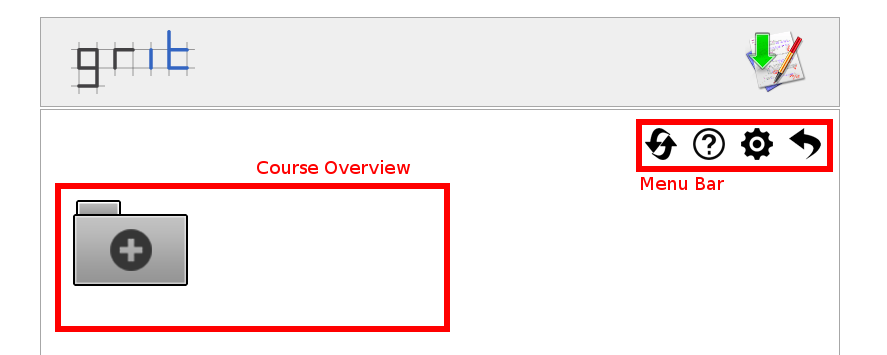
\includegraphics[width=.6\textwidth]{pictures/home.png}
	\end{center}
	Before you start creating new courses you should read section \ref{dataSourceSpecific} because you may need to fulfill external requirements. Now you will need to create a course. For that click on the
        folder with the plus sign.
	\begin{center}
          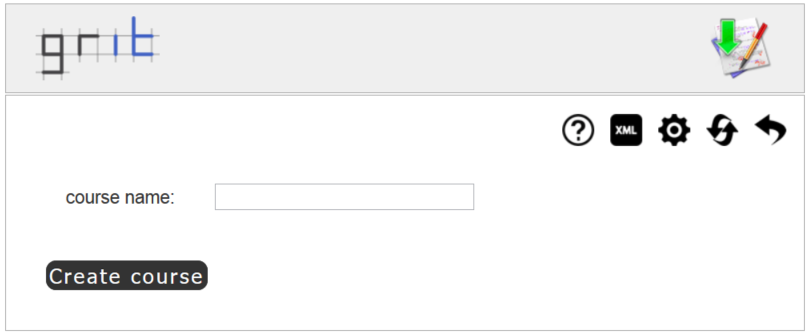
\includegraphics[width=.55\textwidth]{pictures/create_course.png}
	\end{center}
	You will be prompted to enter the course name, after that
        click on {\tt Create course}. The created course will now be
        visible in the overview.
	\begin{center}
          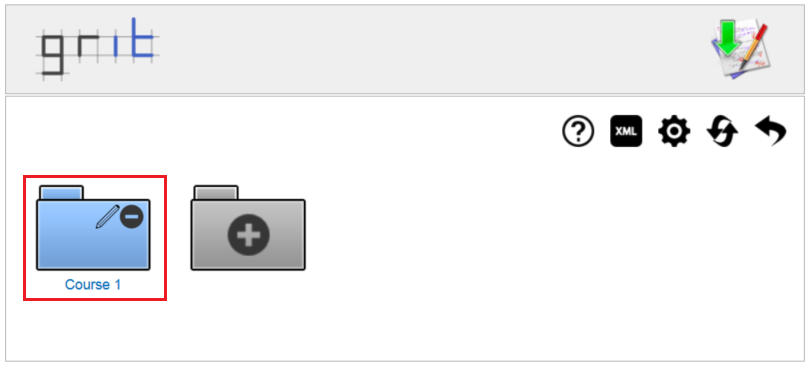
\includegraphics[width=.55\textwidth]{pictures/created_course.png}
	\end{center}For creating an exercise we will first need to set
        up a connection so \product{} knows where to get the students'
        submissions from. For that click on the "gear wheel" symbol in
        the menu bar. You get now presented the connection overview.
	\begin{center}
          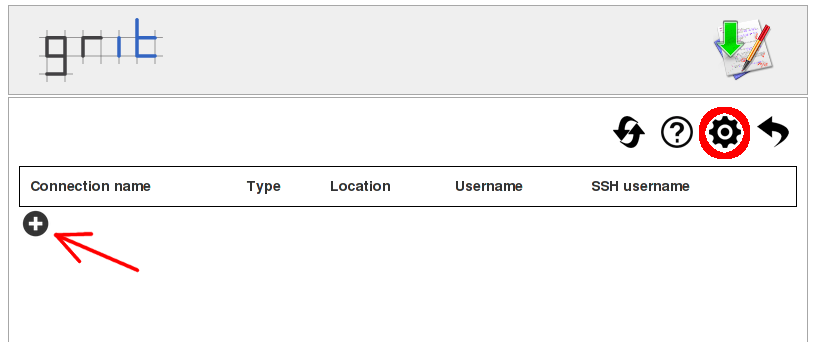
\includegraphics[width=.55\textwidth]{pictures/connection_overview.png}
	\end{center}
	To add a new one click on the plus sign. You will get to a
        form where you can enter the connection information:
	\begin{description}
        \item[Connection Name:] Name for you to identify the
          connection.
        \item[Connection Type:] Either, ILIAS, SVN or Mail is
          suuported as of \product{} \version.
        \item[Location:] The {\tt url} of the root folder where the
          submissions will be.
        \item[Username:] The name of the ILIAS or SVN account.
        \item[Password:] The password for the ILIAS, SVN or Mail
          account.
        \item[ssh Username:] If you are setting up an ILIAS
          connection, enter the account's user name which is being
          used to copy files from the ILIAS machine.
        \item[ssh Key-File:] The file containing the key which is used
          to authenticate the ssh connection with the ILIAS machine.
        \item[Structure:] The strucure that \product{} will encounter
          so it knows where to get the submission. For more see
          Section \ref{structure}.
	\end{description}
	\begin{center}
          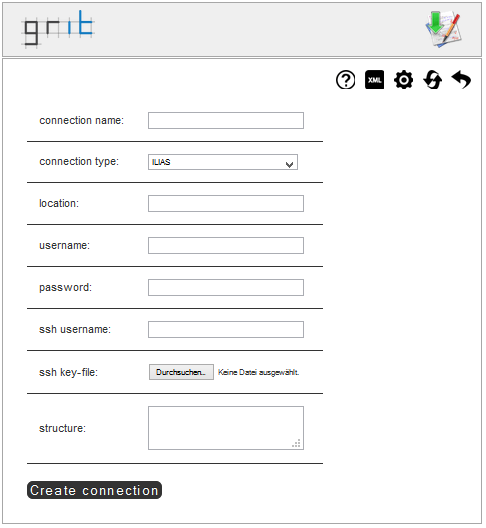
\includegraphics[width=.55\textwidth]{pictures/create_connection.png}
	\end{center}
	At the end click on {\tt Create Connection}. And you will see
        the created Connection in the overview.
	\begin{center}
          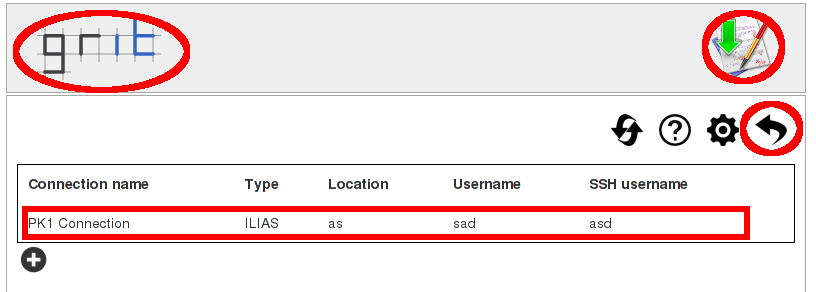
\includegraphics[width=.55\textwidth]{pictures/connection_overview2.png}
	\end{center}
	Now you go back to the course overview. Either by clicking the
        "back arrow" or by clicking the \product{} logo. Now click on
        your created course and you will see the exercise overview.
	\begin{center}
          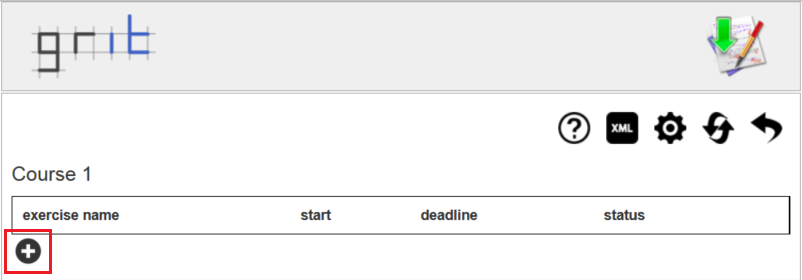
\includegraphics[width=.55\textwidth]{pictures/exercise_overview.png}
	\end{center}
	Similar to the connection overview you can now create a new
        exercise by clicking the plus button and again will be
        prompted a form:
	\begin{description}
        \item[Exercise Name:] The name of the Exercise that will also
          be printed on the output document (i.e. Exercise 1/Übung 1).
        \item[Language:] The programming language for the
          Exercise. Java, C/C++ and Haskell are supported as of
          \product{} \version.
        \item[Start at:] The date the exercise gets handed out to the
          students.
        \item[Deadline:] The date when the students must have
          submitted their submissions.
        \item[Connection to use:] Here you will select the connection,
          previously created, to be used with the exercise.
        \item[Unit Test file:] The (optional) file that contains Unit
          Tests to test for. Only JUnit is supported as of \product{}
          \version.
	\end{description}
	\begin{center}
          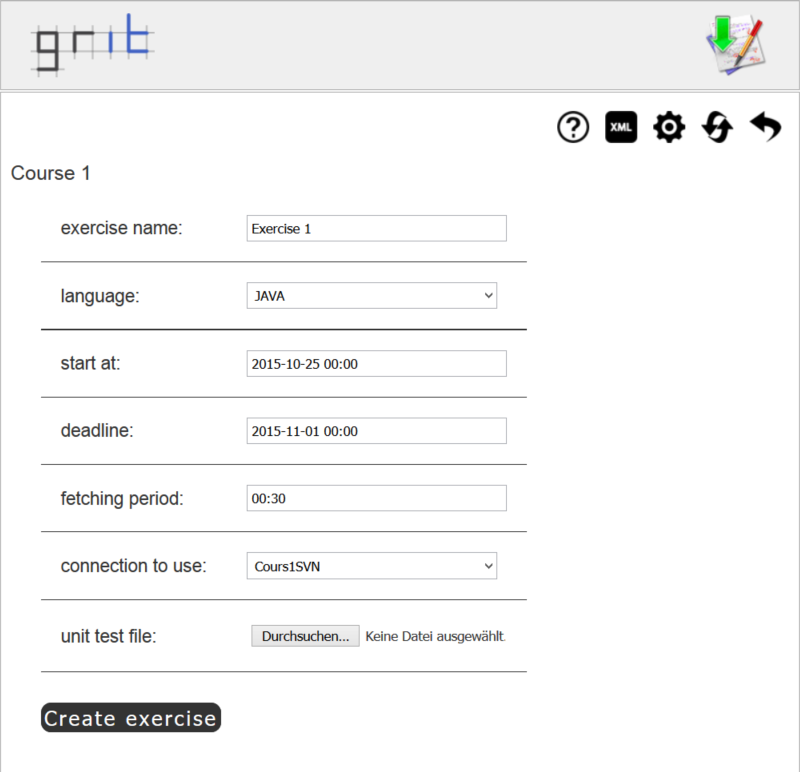
\includegraphics[width=.55\textwidth]{pictures/create_exercise.png}
	\end{center}
	Now you can click {\tt create exercise} and you will see the
        just created exercise in the overview. If you setting made are
        correct everything is set up now and you can wait for the
        deadline. If you made some error you can click the pencil
        symbol to the right of the exercise entry and change the
        settings.
	\begin{center}
          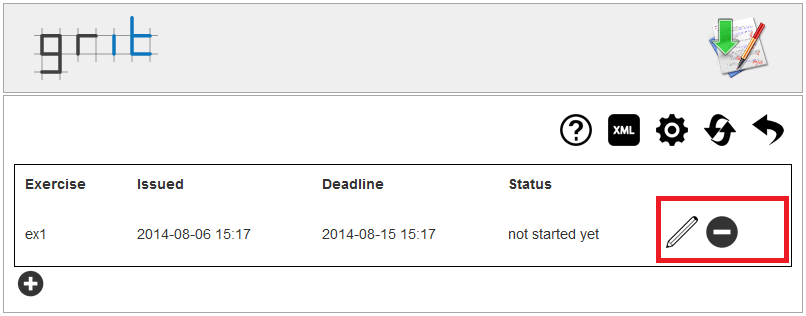
\includegraphics[width=.55\textwidth]{pictures/exercise_overview2.png}
	\end{center}
	Finally the end of the deadline we will process the
        submissions and when finished an additional symbol will be
        visible next to the exercise entry: With that you can download
        the PDF Document containing the students submission, the
        compiler output and - if existing - the test results.

	\section{Setting up a submission structure}\label{structure}
        In order to be able to correctly match student submission
        files to students in SVN repositories, \product{} needs to
        know the structure of the directory tree it is supposed to
        look at. For this purpose you need to enter a comma separated
        list of regular expressions which match the path \product{}
        needs to traverse to find submissions. The special tags
        \texttt{TOPLEVEL} and \texttt{SUBMISSION} indicate the
        repository root and the submission level respectively.

        For example, your repository might have two folders at its
        root: \texttt{exercise/} and \texttt{lecture/}. While the
        latter contains no submissions, \texttt{exercise/} contains a
        folder for each student: \texttt{stud01/}, \texttt{stud02/},
        \texttt{stud03/} and so on. Each of these students has a
        folder for each exercise: \texttt{ex01/}, \texttt{ex02/},
        \texttt{ex03/} and so on.

        In order to tell \product{} to look in a specific folder(e.g. \texttt{ex01})
        you would specify the following list:

        \begin{lstlisting}
          TOPLEVEL
          exercise
          stud[0-1][0-9]
          ex01
          SUBMISSION
\end{lstlisting}

        \texttt{TOPLEVEL} stands for the root of the repository. Then
        \product{} will only look at the \texttt{exercise} folder. In
        there, all folders from \texttt{stud01} upto \texttt{stud19}
        will be inspected. In each student folder \product{} looks at the folder ex01. From
        here the system will retrieve the current submission.
        
	\section{Configuration}\label{config} 
		The config file contains important data for the server, the mail 			notification and the admin account. This information is stored in 		an .xml file located at \texttt{config/config.xml}. If there is 			no config present at boot the standart failsafe config will be 				loaded. This config looks like this:
		\newpage
		\begin{lstlisting}
		<?xml version="1.0" encoding="UTF-8" standalone="no"?>
		<config>
			<server>
				<port value="8080"/>
			</server>
			<email>
				<auth password="" adress="" host=""/>
			</email>
			<admin>
				<user name="username" email="" password="password"/>
			</admin>
		</config>
	    \end{lstlisting}		   
       	The structure consists of the following items:
       	\begin{description}
        \item[<config>:] Wrapper tag which specifies when the config 					starts and when it ends.
        \item[<server>:] Holds info about the server.
        \item[<port>:] The port the server is running on.
        \item[<email>:] Holds info about the email account where the							notification mails are send from.
        \item[<auth>:] All relevant authentication info for the mail account. The password, the mail address and the SMPT host server(e.g. smtp.gmail.com).
        \item[<admin>:] Holds info about the admin account.
        \item[<user>:] The data with which you want to log into the website and the email the admin want to get notifications on.
		\end{description}
		In order to customize the config you just change the values between the quotation marks. To do so please use the respective edit xml function on the webinterface. After the configuration was changed the system needs to be rebooted. This will be done automatically in the edit xml function. You should especially consider this if you changed the config file without the edit xml function on the webinterface.
       \section{Data Source Specific Requirements}\label{dataSourceSpecific} 
        There are some things you need to consider when creating courses and exercises.
       \subsection{Ilias}
       If you create a new course witch will be using an ILIAS connection for an exercise you need to meet some requirements. At first the mapping from \product{} to ILIAS is that courses in \product{} resemble exercises in ILIAS and exercises in \product{} resemble assignments in ILIAS. This is due to the internal database schema of the ILIAS data management. Now you have to make sure that before you create a new course or a new exercise in \product{} this courses and exercises already exist in ILIAS. If not fetching will not work properly. They also need to have exactly the same name. For example:\\\\
	    \begin{tabular}{c c | c c}
	    GRIT: 				&		& ILIAS:				& \\\hline
	    Course: 			&PK1	& Exercise: 			&PK1\\
	    Exercises of PK1:	&ex1	& Assignments of PK1:	& ex1\\
	    					&ex2	&						& ex2
\end{tabular}	 \\\\
Furthermore you should ensure that there are no ambiguities in the name schema of the courses and the exercises so that exercises can be clearly distinguished. For example you should not have two courses with the exact same name.
  	
       \subsection{SVN}
       For SVN you have to make sure to choose a different connection
       for every exercise because the submission structure in the
       connection specifies which exercise you want to fetch from the
       repository.

       \subsection{Email}
       If you decided to use email submissions, you already have
       specified the email address from which \product{} should fetch
       email submissions. In order for this to work as intended,
       students have to name the email subject according to the
       following formula:

       \[ \texttt{[course name-exercise name]} \]

       E.g. when the course name is ``Programmierkurs 1'' and the
       exercise name is ``1'' (for the first exercise), then the
       subject should be \texttt{Programmierkurs 1-1} so \product{} can
       find the submission. Also consider that submissions handed in
       after the dead line are not imported.
       
	\chapter{Frequently asked Questions}
	\begin{enumerate}
        \item \textit{What does \product{} do?}
		
          \product{}  assists you in running a programming course where
          it is required for students to hand in assignments done in
          code. The submissions can be automatically fetched from
          associated repositories and automatically tested. \product{} 
          delivers a well-structured and comprehensive document ready
          to be graded by a corrector as well as overall and detailed
          course statistics.
		
        \item \textit{What does \product{} not do?}
		
          \product{}  integrates between the steps assignment issuance,
          submission and correction. To be precise, it fills the
          formerly manual between submission and correction, as well
          as everything that comes after correction. \product{} does not
          provide facilities to issue assignments, submit them, and,
          certainly cannot correct them.
		
        \item \textit{On what type of machine should I install
            \product?}
		
          As the provided virtual machine is very light-weight, any
          computer with constant internet access and at least 1GB
          memory for the VM does the job. However, we encourage you to
          use a dedicated server machine and not your personal
          computer to run the \product{} back-end.
		
        \item \textit{Do I need a virtual machine for \product?}
		
          It is possible to install the \product{} back-end without any
          virtualization software or virtual machine. However, we
          strongly suggest using a virtual machine due to security
          concerns. Furthermore, we only provided comprehensive guides
          for using the virtual machine, this, if you wish to go
          without one, you are on your own.
		
        \item \textit{What is the default username and password?}
		
          The default username is {\tt username} and its password is
          {\tt password}.
		
        \item \textit{What is the {\tt root} password?}
		
          The {\tt root} password is {\tt root}
		
        \item \textit{Should I change the predefined passwords of the
            provided VM?}
		
          Yes.
		
        \item \textit{Is it possible to use a graphical user
            interface?}
		
          If you wish to run \product{} natively or on another virtual
          machine, you will find the associated requirements in
          \hyperref[4.3]{Section 3 of Chapter 4}.
		
	\end{enumerate}
	\chapter{Credits}
	\section{Developers}
	\begin{itemize}[label=]
        \item Gabriel Einsdorf
        \item Marvin Gülzow
        \item Eike Heinz
        \item Marcel Hiller
        \item David Kolb
        \item Fabian Marquart
        \item Thomas Schmidt
        \item Stefano Woerner
	\end{itemize}
	\section{Special Thanks}
	\begin{itemize}[label=]
        \item Arno Scharmann
        \item Dr.-Ing. Ernst de Ridder
        \item Sigmar Papendick
        \item Simone Winkler
        \item Tino Klingebiel
	\end{itemize}
      \end{document}
